\chapter{如何做好准备} % Introduction chapter suppressed from the table of contents

\hypertarget{ux5206ux6790ux4e8bux6545ux6839ux56e0ux4e0bux96c6}{%
\subsection{分析事故根因:下集}\label{ux5206ux6790ux4e8bux6545ux6839ux56e0ux4e0bux96c6}}

我:陈总,听说你三年前开始锻炼马拉松,所以现在身体这么好,有什么心得可以让我学习一下?\\
总经理:本来我很胖,也常常很困,体检指标不太理想,我听说可以用长跑锻炼身体,便开始尝试。开始的时候并不容易,因为一直都没有锻炼,先跑五六公里,按程序逐步提升,后面便慢慢养成习惯。最终经过三年锻炼完成马拉松,身体也觉得比以前好多了。\\
我:开始的时候,请问您怎么去持续维持,因为很多人还是一时冲动去锻炼,但持久不了,例如买了跑步机,但一两次后面就没再用了,您有什么心得可以让你持续下去?\\
总经理:现在支持长跑运动员的度量挺多,最简单的指标就是一公里要多少分钟。我就一直都有度量这个系数来监控进展。比如我开始的时候一公里要接近八分钟,跟走路差不多,后面慢慢就变成七分钟,六分半,六分钟。。。是锻炼出来的,所以有了这个数,我就知道自己现在是什么水平,是否在进步。\\
我:好比每天跑步锻炼,如果没有手表帮你度量时间速度,你是不知道是否有进步;数据可以给做事的人反馈,让当事人知道现在在差距有多少,所以如果可以从定性提升到定量管理,也可以产生同样的作用。例如,:如果评审发现缺陷数量太少,团队应该担心,因为很可能有不少缺陷未被发现,后面到了客户使用时才暴露,代价更大。感兴趣吗?\\
总经理:很感兴趣。\\
我:首先须要利用以往项目数据,建立标杆(基线)例如下图:

%\href{文件:微信截图_20230605130227.png}{500px\textbar{}无}

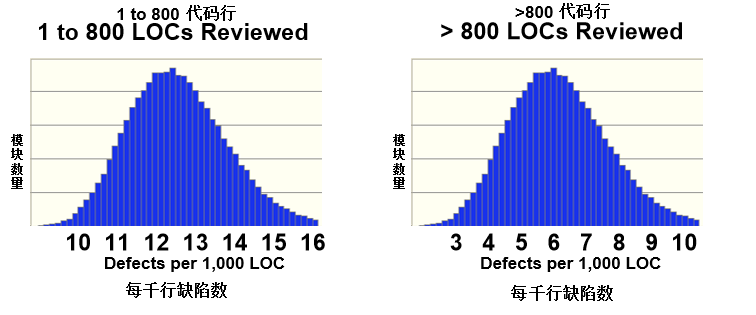
\includegraphics[width=6cm]{微信截图_20230605130227.png}

如果代码是800行以下,每千行代码的缺陷密度均值与范围。800行以上的缺陷密度会低一些,因分母较大。\\
如果某次代码评审,700行的模块,代码评审发现的2个缺陷,比基线下限7个缺陷(注)低很多,团队便应担心,很可能存在不少缺陷未暴露。\\
总经理:但我希望团队有提升,不仅仅是维持,团队怎样可以利用度量数据帮助提升?\\
我:可以利用水晶球模拟,利用缺陷排除率,预估如使用新方法后的缺陷范围。\\
如果也收集团队的缺陷返工工作量,我们更可以预估能降低多少返工。
从降低后面缺陷返工入手,能提高产品开发质量,也能提高团队的生产效率,降低开放成本\\
注:从基线左图,如按每千行代码有10个缺陷为下限,700行代码便应发现起码7个缺陷

\framebox{%
\begin{minipage}[t]{0.97\columnwidth}\raggedright
我用实例在白板上估算提前发现解决缺陷能降低研发成本接近一半。\strut
\end{minipage}}

总经理:很好,应怎么样开始?\\
我:你们有没有团队已经是按迭代开发? \\
总经理:有的,我们去年开始已经有些团队按一个月一个迭代交付,有些更短可能两到三周。\\
我:你们这些团队人员的能力主动性如何?\\
总经理:我觉得还是挺不错的。\\
我:如果你可以识别出两到三个正在在迭代开发的团队,就可以开始做量化的回顾,你们那些迭代团队以前有每轮迭代后做回顾的习惯吗?\\
总经理:都没有。\\
我:首先就要让他们了解什么是根因分析?为什么要做回顾/复盘?希望达到什么目的? 你们管理层也需要有心理准备。开始的时候人员要花时间学习,因为你们也准备参加CMMI评估,团队做好量化迭代回顾就可以帮助你们从三级水平提升到CMMI4级,并开始利用项目迭代数据,建立基线和预测模型。但团队要做好第一次迭代回顾,就像要小孩学游泳,不能只是扔他到水池里面要他自己自学,必须先有培训帮助他。首先要安排这些团队参加根因分析和回顾培训,也需要你们内部的管理层包括有经验的主管作为内部教练,辅导团队,你们愿意尝试吗?\\

\begin{description}
\tightlist
\item[]
= = =
\end{description}

有了高层的支持,我们便可以试点,找团队做好迭代回顾,但不会是立马点石成金,是持续改进过程。

要利用根本原因分析做改进,必须有数据, 也需要有机会立马实验改进方法,评判效果, 所以迭代回顾(或复盘)是做根本原因分析的最佳时机。 但很多团队只在迭代回顾时讨论如何解决迭代暴露的缺陷与相关职责分工,没有探索根本原因, 和如何能避免同类问题再发生。

想了解如何做好回顾,先看回顾的主要步骤:

\hypertarget{ux56deux987eux6d41ux7a0b}{%
\subsection{回顾流程}\label{ux56deux987eux6d41ux7a0b}}

冲刺回顾可按下图的五步,确保各成员都全心投入参与,并能从分析形成行动,达到改进效果:\\


\begin{enumerate}
\tightlist
\item
  设置舞台 --`破冰'
\item
  收集数据(除了收集”硬”数据,如缺陷,工作量,进度偏差等,也要收集”软”数据,如团员感受)。
\item
  分析,找出根因
  (除了鱼骨图,FMEA、也可参考附件里的KJ分析法,大家利用便利贴做分析)。
\item
  决定做什么 (必须明确下个迭代的具体改进行动到人、任务、时间)。
\item
  结束。
\end{enumerate}

%\href{文件:RetrospectiveScreenshot_2021-09-21_173119.png}{500px}

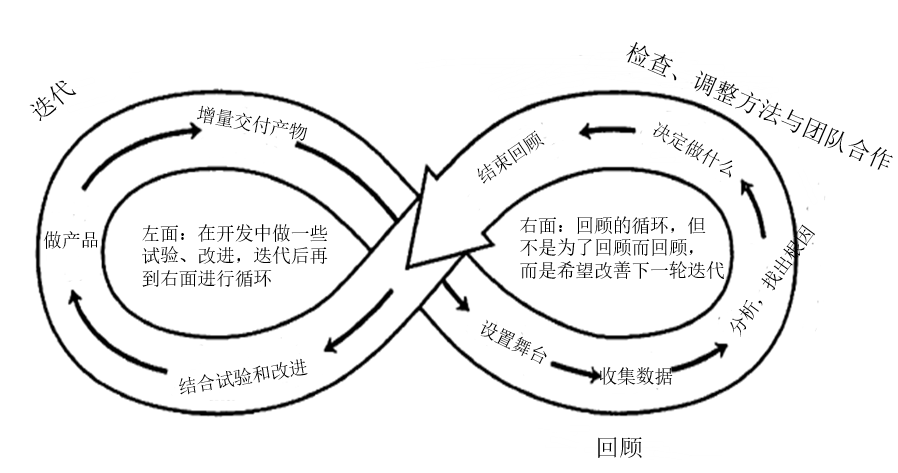
\includegraphics[width=6cm]{RetrospectiveScreenshot_2021-09-21_173119.png}

以上只是根因分析的技巧,若要团队做好迭代复盘,取得效果,还要注意以下原则:

\hypertarget{ux505aux597dux56deux987e4ux539fux5219}{%
\subsection{做好回顾4原则}\label{ux505aux597dux56deux987e4ux539fux5219}}

1. 回顾让数据提供者能即时收到反馈\\


\begin{itemize}
\tightlist
\item
  软件开发与工业生产不一样,大部分的数据必须开发人员自己收集,不能但靠机器/系统(例如:返工工作量)
\item
  如果回顾时分析根因是依据迭代数据,除了能帮助根因分析更具体外,也让团队成员有动力收集数据(因他们知道会一起分析数据)
\end{itemize}

因为软件开发是知识性工作,例如,某活动所花的工时,必须靠个人记录(具体步骤可参考`个人量化管理')

\begin{itemize}
\tightlist
\item
  但记录数据要花精力,如果不了解收集的数据,后面有什么用途,便难以维持不断收集数据的习惯
\item
  反之,当大家都清楚到迭代回顾时会一起分析团队数据,并制定针对改进措施,就有动力继续迭代里统计数据
\end{itemize}

2. 整个团队(所有相关干系人)参与\\
整个团队分析全局问题。例如,如果只是从测试人员的角度,他可能以为缺陷都是来自开发;需求分析人员(或产品经理)会觉得自己做得很好,因需求评审里没有什么问题被发现。但如果团队所有成员聚在一起(包括项目经理、需求、设计、编码、测试),把所有的缺陷列出来,让团队所有岗位一起分析,才可以全局看问题,才可能发现不少问题是因为需求没有明确,导致后面做出来的功能并不是客户要的。后面可扩大参与回顾的干系人,例如客户代表,可以更全面分析。\\
3. 让团队自己寻找改进方案 \\

\texttt{~必须参与一起分析、讨论,才有动力后面采取行动。}

\framebox{%
\begin{minipage}[t]{0.97\columnwidth}\raggedright
``我们团队回顾都是全部成员参加,一起讨论''某团队组长说。
以下是团队一起讨论后的根因分析结果:

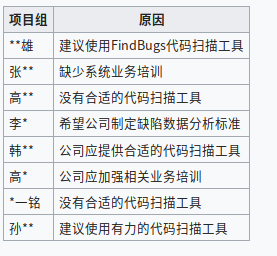
\includegraphics[width=6cm]{Screenshotfrom2023-10-3104-24-58.png}


有没有看到组长提出建议使用代码扫描工具后,其他7位团队成员中4位也提类似原因?\\
所以当团队一起围着开会时,很多人都会避免提出与众不同意见,所以如果用投票方式,让大家对提出的``原因''进行投票时,票数最多的通常也是组长提出的方案(扫描工具)。
\strut
\end{minipage}}

从Asch
1951实验(详见附件),看到人容易受群众压力影响(尤其当大家不认识),不敢独立表达个人看法,所以很多会议都只是项目经理一言堂,其他人只是观众,没有投入分析。
为了鼓励每人畅所欲言,表达独立看法,并达到共识需要:

\begin{enumerate}
\tightlist
\item
  鼓励每人用实例讲对质量、过程的观点/经验(寻找大家的共通点)。
\item
  鼓励每人分享个人感受,想法,满意开心/困惑的时刻(让大家相互了解)。
\end{enumerate}

\begin{itemize}
\tightlist
\item
  当大家感受到都是面对类似的问题,才会放开自己,分享个人看法。
\item
  教练的目标是让每人都有充分机会表达自己的观点。
\end{itemize}

所以在回顾时,也要想办法避免发生这种心理上的影响,导致不能真正挖掘问题的原因。所以在回顾需要大家开放,以下两方法可以减少团队压力,让大家更投入,能畅所欲言:

\begin{enumerate}
\tightlist
\item
  回顾开始时
  (设置舞台,``破冰''),用互动游戏,让团队放开顾虑,全心投入讨论
  (可参考附件里``游戏:应与否'')。
\item
  KJ分析法(详见附件):每人都有一支水笔+便利贴 ,一起找根因,每人都可以写上自己的意见。而不是传统开会方式。很多时候都只是某人讲,其他人听。无法得到团队成员充分参与。如果可以给团队自主权,他们就更能发挥、更能达到目标。\\
\end{enumerate}

如果能让每位团队成员都有充分机会表达意见,不单能集思广益,做到更好的对应方案,也能提升团队后面执行改进方案的积极性,因为一般人都会更喜欢自己的选择。

详见附件里两个实验:

\begin{enumerate}
\tightlist
\item
  Brehm 1956 决策影响实验
\item
  粮食分配实验
\end{enumerate}

%验证了:人都会觉得自己选的东西比较好,更有动力尝试。

4. 看全局,寻找大家的共同点\\
避免局部最优(sub-optimization),避免盲人摸象,
最终希望可以全面从每个角色的视角全面分析。

某公司管理层一直非常关注度量,对各过程,包括需求、开发、测试等,都订了七八个KPI指标,并每月监控。但各个过程按指标做好不一定代表总体效果会好。
每个过程都会影响软件开发最后遗漏到客户的缺陷数,迭代回顾的时候,团队可以用缺陷排除的预测模型让团队`看见'如果代码评审排除率提升如何影响每个过程的缺陷数,不仅仅是定性的讨论分析。

例如,为什么要用`设置舞台'开始迭代回顾?(例如`应与否'是其中一种方法,详见附件),目的是让整个团队全心参与,如大家没有担心,愿意提意见,才能更全面看问题,寻找共同点,而不是辩解。

\framebox{%
\begin{minipage}[t]{0.97\columnwidth}\raggedright
例如发现大量缺陷大部分都在系统测试和验收测试才暴露,
大部分缺陷未在前面评审和单元测试发现并解除,根因分析讨论后发现单元测试没有任何要求,依赖程序员自己测。但很多时候程序员就因为时间压力都没认真去测。因为大家都忙,没有时间去深入去看,代码评审也没有发现多少问题。针对这些点大家觉得可以加强静态扫描工具,尽早发现一些语句基本问题,或重复代码等问题,减轻依赖人工查看;单元测试可以用脚本写,并规定有一定的语句覆盖率要求(例如,\textgreater{}80\%)。但如果团队只是按这些去做,没有定量化目标就很难衡量,做得够不够?不然要等到迭代最后复盘时才知道效果如何。

好比要设计一座新的80层高楼,建筑师预先用工程模型预估它防地震、防台风的能力,不要等到建好才知道有问题。团队可利用蒙地卡罗预测模型预先依据以往迭代的数据,把参数输入模型,比如每个阶段引入的缺陷数,每个阶段的缺陷排除率。首先可以利用蒙地卡罗模型,看看它出来的缺陷分布,验证是否对应以往迭代数据,预估范围是否可以覆盖以往数据。

第二步,就可以使用蒙地卡罗模型做一些实验:例如,我们估计用了静态扫描可以把代码评审的排除率从本来的10\%提升到50\%,团队利用蒙地卡罗模型可以预估这种搭配的各个过程的缺陷分布,我们就可以看到如果这个排除率提升的话,评审应该出发现多少缺陷,比以往提升多少。团队也可以加入利用脚本的单元测试的缺陷排除率,例如估计能从本来的排除只有20\%提升到55\%,看到对整个缺陷分布的变化?这样的话,我们就可以团队有下一轮迭代各个过程的缺陷预估范围参考。如果发现在代码扫描后这个缺陷数达不到本来的预期目标,便可立马采取纠正措施,不要等到最后迭代回顾时才发现未能达不到本来的预期效果。

如果有好几种方法选择,蒙地卡罗预测模型更可以帮我们做选择一个最优的最佳搭配,比如我们只是先做好评审,还是先做好单元测试,因为那些都会增加一些工作量,还是两边种方法都做,我们就可以要用蒙地卡罗以总成本最低选最佳搭配。反过来,如果没有这种蒙地卡罗工具的话,团队是很难看到每一种变化总体的效果,像盲人摸象。

因为工具可以反映过程之间的相互关系,如果我前面评审发现多了,遗漏到后面的缺陷就会减少,一层一层的关系,它利用那个缺陷排除的关系模型就可以估计总体的效果,也帮团队迭代回顾从定性改进分析,提升到定量。(如何从迭代的缺陷数据,利用蒙地卡罗预测模型,做定量分析,详见附件。)
\strut
\end{minipage}}

\hypertarget{ux56e2ux961fux8fedux4ee3ux56deux987eux6839ux56e0ux5206ux6790ux5e38ux89c1ux95eeux9898}{%
\subsection{团队迭代回顾根因分析常见问题}\label{ux56e2ux961fux8fedux4ee3ux56deux987eux6839ux56e0ux5206ux6790ux5e38ux89c1ux95eeux9898}}

\begin{enumerate}
\tightlist
\item
  没有利用缺陷数据做帕累托图分析,不清楚应针对哪一类,不清楚哪一类问题最多,导致根因分析讨论没有针对性。有些缺陷分类没有定义好,不明确或重同一缺陷可以归到几个类别,导致分析结果没有参考作用。
\item
  不清楚怎么是根因,只找到表面看到的现象,例如人经验不足,对技术不熟悉,对业务不熟悉等。没有抓到系统的根本问题。
\item
  没有量化目标,只有定性的根因分析,下轮迭代难以判断效果能否达到。
\item
  回顾时间不够。
\item
  设备、纸张、工具等未准备好。
\end{enumerate}

\framebox{%
\begin{minipage}[t]{0.97\columnwidth}\raggedright
除了教团队根因分析技巧(定性)以外,也需要展示如何使用水晶球蒙提卡罗预测模型,预估各类缺陷数范围,有了范围才可以判断最终结果是否达标,差多远。识别出哪些过程有差异,下一轮回顾才能更有针对性。如果团队想下一个迭代降低遗漏到客户的缺陷数,尽量提前用评审或测试预先发现并解决。如果仅仅提一些改进方法,比如加强评审,使用工具等,效果很有限。例如团队一般也有做评审,例如需求评审,但无法判断评审质量如何? 例如,发现四个缺陷是否足够呢?我们就可以用缺陷排除率配合蒙地卡罗模型,估计使用新提升方法后,预计的缺陷数范围,这样的话,如果团队发现缺陷数没达到预期,就知道立马可以加大力度加强,而不仅仅是走过程。(关于缺线排除率配合蒙地卡罗的原理,详见附件)
\strut
\end{minipage}}



以上前三点可以利用培训加强相关能力,为了确保团队能做好第一次迭代回顾,建议要之前和团队做培训。
后两点可以做好准备,预防问题发生,所以若要做好回顾,除了要理解上面4原则,也需要注意以下两条件:

\begin{itemize}
\tightlist
\item
  回顾的环境、设备: 有大白纸贴在墙上、水笔、便利贴等。
\end{itemize}

\framebox{%
\begin{minipage}[t]{0.97\columnwidth}\raggedright
有时便利贴可能太小,或字很小,原因是如果用一般的白板笔,字就太大了,如果用平常的0.5mm水笔,太细,字太小,都不合适。应该买一些比如2MM粗的水笔,才合适写便利贴。让大家可以在一到两米距离都能看得清。还有那些便利贴是不适合直接贴在普通白板上的,所以必须先从图文店买一卷比如两米宽的卷纸,用泥胶稳固在墙上;因便利贴只是上边有粘性,要在便利贴下部背面贴上一点泥胶,便不会出现便利贴下面翘起来,影响整个KJ报告看不清的情况。整个房间应该有充分的空间让大家活动,而不是那种传统一个大长座的会议室,因为越是让大家活动流动,才能投入。\\
\end{minipage}}

\begin{itemize}
\tightlist
\item
  足够的时间,起码3小时。
\end{itemize}

\framebox{%
\begin{minipage}[t]{0.97\columnwidth}\raggedright
某成都客户反馈 研发总监:
已经做了很多年过程量化考核,起初能给团队带来活力,因为至少比以前好,有路径可以量化他们,员工觉得做有所值,公司也看得见。前几年执行的很好,产出和上线频率比过去好很多。但是现在感觉逐渐拉不出差距来,因为大家都非常熟悉这套游戏规则。

我:理解,比如现在你们团队开始做迭代回顾,团队一起分析根因,持续改善。您觉得效果如何?

研发总监:挺好,但是还是感觉他们开回顾会,耗时太长了,2个小时以上

我:因需要团队收集数据,分析,讨论下迭代措施,所以通常要3小时,熟练后会快一点,底线是改进的节省应大于回顾的投入。

高层的支持是任何改进的重要成功要素。所以首先要让管理者赞同迭代回顾能为公司带来回报(省钱),可以节省的成本(工作量)大于回顾的人力投入;也要让他理解任何改变都有个混沌的过渡期,要经过几轮回顾后,团队才能自己持续改善。
\strut
\end{minipage}}

\framebox{%
\begin{minipage}[t]{0.97\columnwidth}\raggedright
如果回顾只能一个或一个半小时的话,就不够时间让团队针对缺陷分组分类、画帕累托图做分析,没有根据实际数据分析根因,也影响到团队没有动力在后面迭代花精力去收集数据。例如,缺陷返工数据一直都非常难获取得到的,也需要在迭代根因分析时给时间团队讨论统计,所以通常一个完整的迭代根因分析回顾不会小于三小时。要做好这块如果有本地的教练可以更好控制整个回顾的节奏。不会在某一个环节耽误太多时间,也不会太长,也确保大家团队人员都全程投入讨论参与。这个我们在下一章会详细讲。
\strut
\end{minipage}}

\hypertarget{ux57f9ux8badux7b56ux5212ux4e0eux51c6ux5907}{%
\subsection{培训:策划与准备}\label{ux57f9ux8badux7b56ux5212ux4e0eux51c6ux5907}}

培训能让团队能先了解利用模拟工具量化管理的原理,也让团队为收集迭代数据做准备,所以建议先做模拟互动培训。

培训的目的:

\begin{enumerate}
\tightlist
\item
  让团队用模拟数据体验一个迭代回顾量化的应如何进行。
\item
  知道为什么要收集缺陷和返工工作量的用途。并利用类似一般开发项目的环境的缺陷数据模拟。
\item
  收集到团队真实数据是最大的挑战,培训过程中也要团队自己讨论准备如何收集迭代的数据。因为没有数据是无法做量化的迭代回顾。
\end{enumerate}

下面是一天互动培训的时间安排:(上午是做上一章迭代回顾的互动练习,下午是使用蒙特卡洛预测模型预测下迭代的互动练习。)

%\href{文件:微信截图_20230830093612.png}{500px}

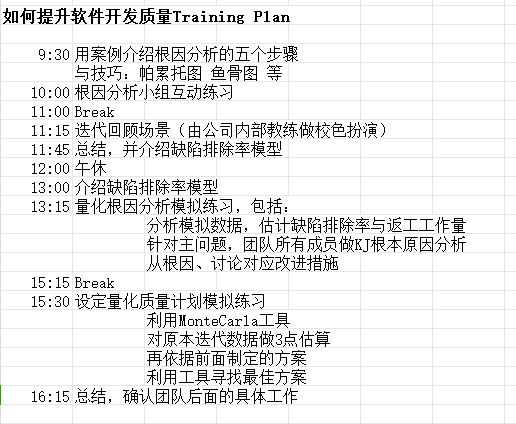
\includegraphics[width=6cm]{微信截图_20230830093612.png}

\hypertarget{ux65f6ux95f4ux5b89ux6392}{%
\subsubsection{时间安排}\label{ux65f6ux95f4ux5b89ux6392}}

如果是首次根本原因分析培训,建议先在培训当天早上做以下根因分析小组互动练习,让大家先熟悉根因分析的重点:

\begin{itemize}
\tightlist
\item
  提供一对模拟数据,要求团队利用帕累托图加鱼骨图分析,找出根本原因与改进措施。
\item
  目的:让团队先感受如何基于数据,找出根本原因。
\end{itemize}

\hypertarget{ux57f9ux8badux5bf9ux8c61}{%
\subsubsection{培训对象}\label{ux57f9ux8badux5bf9ux8c61}}

\begin{itemize}
\tightlist
\item
  后面会参与试点的项目组,培训后可以把学过的在项目里实践。
\item
  所有团队角色都参加。
\end{itemize}

\hypertarget{ux51c6ux5907ux6570ux636eux8ba9ux56e2ux961fux6a21ux62df}{%
\subsubsection{准备数据,让团队模拟}\label{ux51c6ux5907ux6570ux636eux8ba9ux56e2ux961fux6a21ux62df}}

要做量化根本原因分析就必须要有数据,所以内部教练须要预先准备下面缺陷与返工工作量数据,类似一轮冲刺后的场景:

\begin{enumerate}
\tightlist
\item
  系统测试缺陷数据,建议从缺陷管理工具里抽取,40 - 60 项。
\item
  开发个人系统测试BUG返工工时统计表:那个BUG号 / 总修复工时 / 备注。
\item
  开发个人开发期间用于修复评审/单元测试返工工时统计表:那个模块 /。
  总修复工时 / 备注
\end{enumerate}

\begin{itemize}
\tightlist
\item
  打印以上的数据表,发给团队做练习时参考
\end{itemize}

例如,互动练习时,要学员利用开发人员工时表
(模拟他们迭代中用于改缺陷的工时,与评审缺陷数,与开发和修正代码的工时):

%\href{文件:缺陷表4.1.jpg}{500px}

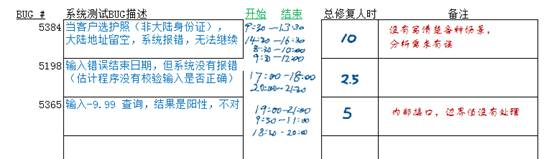
\includegraphics[width=6cm]{缺陷表41.jpg}

%\href{文件:缺陷表5.1.jpg}{500px}

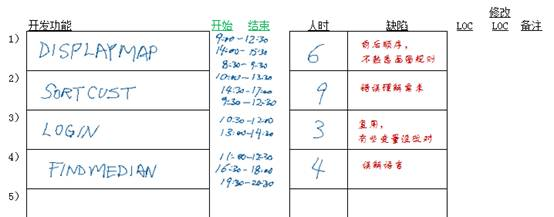
\includegraphics[width=6cm]{缺陷表51.jpg}

\hypertarget{ux51c6ux5907ux5de5ux5177}{%
\subsubsection{准备工具}\label{ux51c6ux5907ux5de5ux5177}}

\begin{itemize}
\tightlist
\item
  分2-4组,6-8人一组,,需要有一个大而光亮的会议室,
  方便小组互动,大白板和架子,各种颜色的水笔,墙壁可以贴上小组的白纸。
\item
  教练提供有MonteCarlo工具的笔记本电脑。
\end{itemize}

\hypertarget{ux4f7fux7528ux4e8cux516bux539fux5219ux4e0ekjux5206ux6790ux6839ux56e0ux5b9eux4f8b}{%
\subsection{使用二八原则与KJ分析根因实例}\label{ux4f7fux7528ux4e8cux516bux539fux5219ux4e0ekjux5206ux6790ux6839ux56e0ux5b9eux4f8b}}

\hypertarget{ux516cux53f8ux80ccux666f}{%
\subsubsection{公司背景}\label{ux516cux53f8ux80ccux666f}}

多年来,这家公司一直做医疗IT解决方案,门槛很高,不仅要懂IT,也要懂行业知识。医院,或医疗机构,都对质量有要求。\\
工作压力也很大 ------
去年业务扩展很快,除了要增加软件产品数量以外,也非常注意产品质量。
例如,公司用系统统计客户反馈的缺陷。要求过程改进小组,按月统计客户反馈的缺陷,看是如何逐步到得到改进、不断完善。因员工人数快速增加,公司也注重控制成本,如研发成本。

\hypertarget{ux4eceux9879ux76eeux51b2ux523aux7684ux56deux987eux590dux76d8ux5f00ux59cb}{%
\subsubsection{从项目冲刺的回顾复盘开始}\label{ux4eceux9879ux76eeux51b2ux523aux7684ux56deux987eux590dux76d8ux5f00ux59cb}}

质量经理把我引到回顾复盘现场,技术总监(高层)也参加,测试人员投影了本次迭代的缺陷分析,展示下面两个缺陷分布图
:

\begin{itemize}
\tightlist
\item
  开发人员排名(最多的排头)
\item
  按模块来区分(最多的排头)
\end{itemize}

团队组长便按照缺陷的严重程度询问每位开发人员 -\/- 是否知道怎么修改?\\
大家都说知道了。组长要求大家提出问题,如果没有问题就准备散会。

我问:大家好,你们有没有兴趣做个小实验。
后面让我们暂时抛开自己本身是什么岗位。
大家一起看看有哪些地方能减少缺陷?

例如,除了按照人员与模块区分。 我们可否把缺陷简单按下面类型分组 :
需求/设计/编码 ?

他们就让测试人员,展示本冲刺发现的34个缺陷,让大家逐一讨论,找出缺陷是源自哪过程
,最后把总数写在在白板上:

%\href{文件:DefectsBySourceScreenshot_2021-09-20_155232.png}{400px}

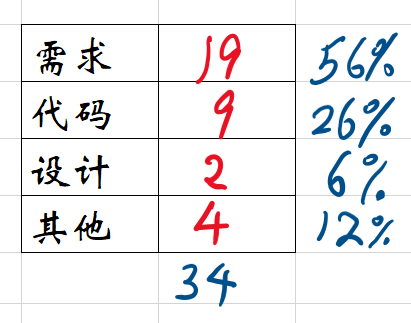
\includegraphics[width=6cm]{DefectsBySourceScreenshot_2021-09-20_155232.png}

让我们看看是怎么分布? 为什么这类缺陷最多呢?大家估计背后是什么原因?
针对需求(最多的类别),我辅导团队利用KJ方法{[}详见附件{]},识别主因。最终汇总成以下结果:\\
%\href{文件:!!reqKJfinal微信图片_20210920125228.jpg}{400px}

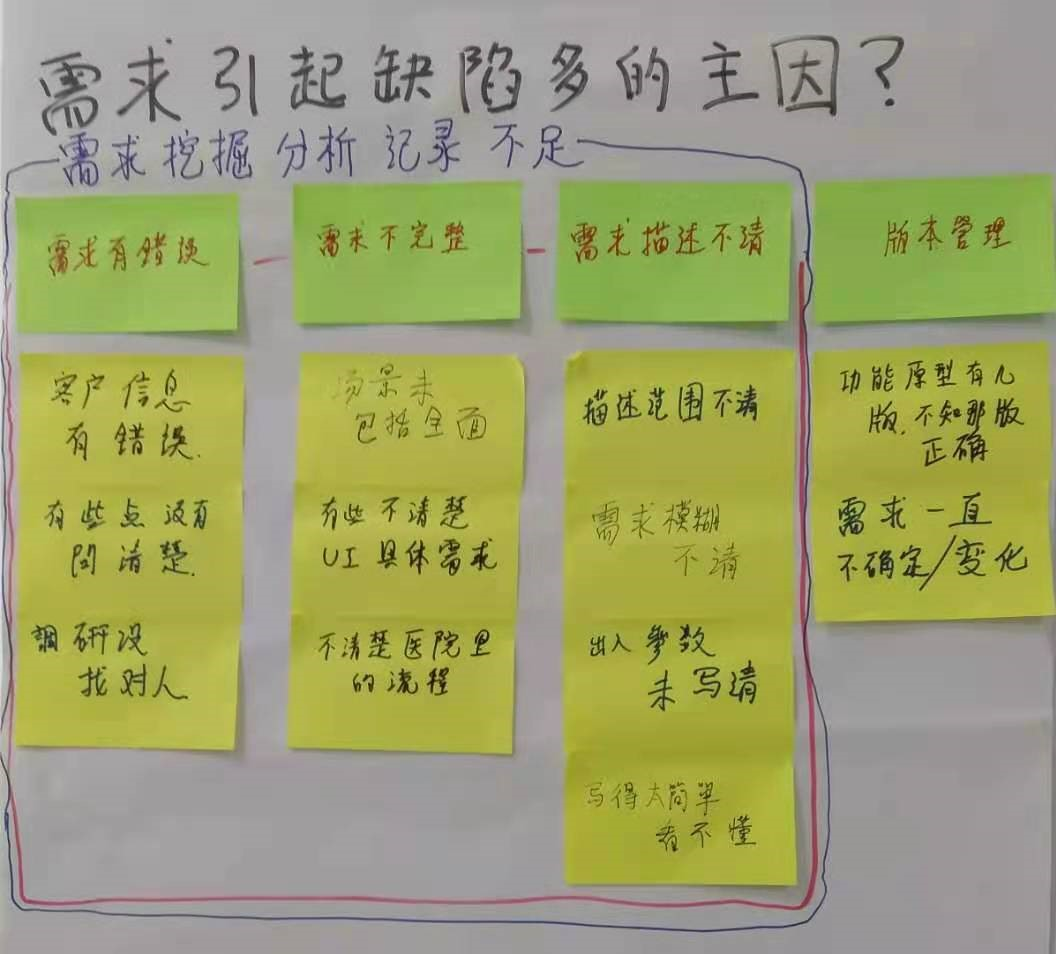
\includegraphics[width=6cm]{!!reqKJfinal微信图片_20210920125228.jpg}

\hypertarget{ux5206ux6790ux95eeux9898---ux6839ux56e0---ux884cux52a8}{%
\subsubsection{分析问题 - 根因 -
行动}\label{ux5206ux6790ux95eeux9898---ux6839ux56e0---ux884cux52a8}}

我:针对我们刚才一起找出的主因,根本原因是什么?
如何可以避免同类缺陷再发生?

总监:要加强对需求人员的培训,提高他们的能力。\\
我年初已察觉到确实很多需求没有表达清楚。
导致开发出来的东西不符合客户要求,或不是客户要的。

总监接下来说:

\framebox{%
\begin{minipage}[t]{0.97\columnwidth}\raggedright
我见过以下用户故事:

病人或他的家属能容易找到他选择的服务。\\
理由:他们熟悉网上购物,习惯了方便和快速的响应时间时间。\\
我问需求人员怎样才算容易找到,验收标准?

我估计她记得我说过需求必须可测量,她想了一会,说:验收标准:``普通病人能够在6秒钟内通过不超过三个动作定位任意一项服务。''

我说如果把`普通病人'改为`90\%以上的病人'更好。

必须把模糊,有二义性的需求变成可以测量。

所以不能仅仅说 `新功能很酷,很创新',
而应明确验收标准为:引入了新功能的三个月之内,60\%的用户应该用它来完成规定的工作。75\%以上的用户对产品表示赞许。

所以三个月前,我已经开始 准备正式规划产品经理与需求分析师岗位:
要经过挑选,考试,然后培训,达标才能正式上岗。
本来计划两周后会正式公告,现在既然你们问到,我就预告一下。\strut
\end{minipage}}

我:既然高层已经有长远的规划,我们团队就应该针对下一个冲刺,我们可以做到的事情。\\
团队:我们每个岗位都已经尽了全力,没有什么可以做了。\\
我:你们有做评审吗?如需求,设计评审\\
团队:有。\\
我:需求评审发现多少缺陷,设计评审发现多少?\\
团队:好像两三个。\\
我:发现什么问题?\\
团队:记不清了,当时直接就修改了。\\
我:请问评审总共花了多少时间?多少人参加?\\
团队:我们六个人,那次评审大概用了接近2小时。\\
我:2小时?\\
团队:我们不仅仅发现需求问题,也一起讨论如何修改\\
我:如果评审只找缺陷,记录,应不会超过一小时,如果大家事前做好准备,估计可能半小时可以完成。所以通常检查(Inspection
)不会当场讨论如何修改。\\
我接着说:我们刚才分析系统测试缺陷,不是识别出超过一半是源自需求吗?为什么我们不能在评审时预先发现?你们觉得可以下一个冲刺,评审时可以发现更多缺陷吗?\\
我立马用5分钟与大家分享有效评审能降提高产品质量,降低成本的例子。

团队:估计应该可以,但不知道怎么做?\\
我:你们评审有检查清单吗?\\
团队:没有。\\
我:清单可以帮助我们吸收以往的经验,避免以后同类问题再发生。例如刚才我们都识别了跟需求挖掘/分析/记录不足相关的具体问题吗?
可否利用这些,更新评审检查单的检查项项,提醒我们要避免同类问题。如果大家同意,我们现在就行动。我们要改进便要制定目标,例如计划下次需求评审,系统测试等各过程发现的缺陷数。这些目标你们可以下周一策划两周冲刺时定。

组长安排了小李更新检查单。准备在下次评审前与需求文档,预先发给参评人员。

我:谢谢大家,我没有其他要说了,下次回顾,我或总监会来参加,看看冲刺的效果。

要利用根本原因分析做改进,必须有数据,
也需要有机会立马实验改进方法,评判效果,
所以迭代回顾(或复盘)是做根本原因分析的最佳时机。
但很多团队只在迭代回顾时讨论如何解决迭代暴露的缺陷与相关职责分工,没有探索根本原因,
和如何能避免同类问题再发生。

\hypertarget{ux7ecfux9a8cux6559ux8bad}{%
\subsection{经验教训}\label{ux7ecfux9a8cux6559ux8bad}}

很多开发人员虽然编码/测试很有经验,但不熟识统计分析,蒙地卡罗模拟等,所以整个培训需要有内部的教练辅助他们怎么利用那些工具技巧去分析数据。团队只是提供数据和分析结果,不一定要很了解里面的数学分析,但必须真正了解根因分析,所以我们培训会以根因分析开始,用前面的丰田故事,日本绅士俱乐部原因分析故事。让大家了解根本原因分析的重点。然后给小组前面的机场延误数据,让他们利用KJ模拟方式和帕累托图,自己动脑筋找出根因,我们的经验:越多互动练习,他们就越感兴趣,越主动参与。所以如果时间有限,尽量可以压缩讲理论的部分,甚至要他自己先阅读了解,大部分时间让他利用数据分析根因。有了这个基础就可以进入第二部分,利用内部教练准备好的几十条系统测试缺陷,要他们按缺陷排除的方式,找出缺陷的主要来源,并估计返工工作量,再利用蒙地卡罗模拟估计每一个过程的缺陷范围。经过培训,他们便可以在下一个迭代回顾时用同样思路,分析自己的迭代数据,找出根因并制定下一轮迭代的纠正措施。培训结束前,内部教练在总结时要求大家团队讨论后面有什么方式可以收集到做迭代回顾所需要的数据,例如缺陷数,返工工作量等。

\hypertarget{ux7ed3ux675fux8bed}{%
\subsection{结束语}\label{ux7ed3ux675fux8bed}}

要做好迭代回顾,首先必须得到高层的支持,并取得所需的资源与时间。策划与培训是成功的第一步。因一般团队没有回顾与根因分析的概念,教练如何现场辅导也很重要。

下章会分享如何在回顾中的注意事项和如何持续。

\hypertarget{ux9644ux4ef6}{%
\section{附件}\label{ux9644ux4ef6}}

\hypertarget{ux6e38ux620fux5e94ux4e0eux5426}{%
\subsection{游戏:应与否}\label{ux6e38ux620fux5e94ux4e0eux5426}}

在迭代回顾中使用。

\hypertarget{ux76eeux7684}{%
\subsubsection{目的}\label{ux76eeux7684}}

帮助建立有效沟通的思维模式。帮助参与者抛开指责和判断,以及对指责和判断的恐惧。

\hypertarget{ux6240ux9700ux7684ux65f6ux95f4}{%
\subsubsection{所需的时间}\label{ux6240ux9700ux7684ux65f6ux95f4}}

8 \textasciitilde{} 12分钟,取决于小组的大小。

\hypertarget{ux63cfux8ff0}{%
\subsubsection{描述}\label{ux63cfux8ff0}}

在描述这些模式之后,参与者讨论这些沟通模式的意义。

\hypertarget{ux6b65ux9aa4}{%
\subsubsection{步骤}\label{ux6b65ux9aa4}}

\begin{enumerate}
\tightlist
\item
  将注意力集中在``应与否''(见下图),并简要阅读。
\item
  组成小组,每组不超过4人。要求每组用一对词来定义和描述。如果有四对以上的词对/组,如果有多个组有相同的词对,也可以。
\item
  让每个小组讨论他们的两个单词的意思和它们所代表的行为。让他们描述各自对团队和回顾的影响。
\item
  每个小组向整个小组汇报他们的讨论情况。
\item
  询问大家是否愿意使用左面的方式。
\end{enumerate}

\href{文件:_游戏1应与否1.png}{500px}

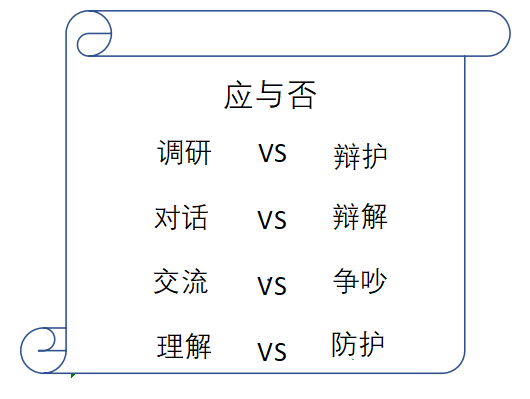
\includegraphics[width=6cm]{游戏1应与否1.png}

\hypertarget{ux7528ux89d2ux8272ux626eux6f14ux4e3aux505aux597dux56deux987eux6253ux57faux7840}{%
\subsubsection{用角色扮演为做好回顾打基础}\label{ux7528ux89d2ux8272ux626eux6f14ux4e3aux505aux597dux56deux987eux6253ux57faux7840}}

学员用各种角色扮演什么是吵架,什么是交流,让观众和表演者更能感受到量化回顾先要有对事不对人的心态:


%1498.png\textbar{}对话 1499.png\textbar{}辩解

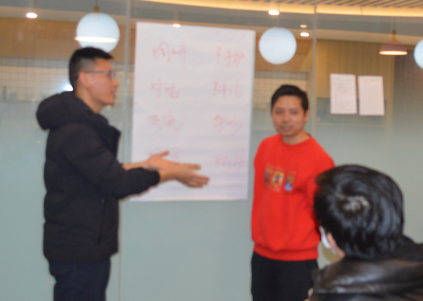
\includegraphics[width=6cm]{1498.png}\textbar{}对话 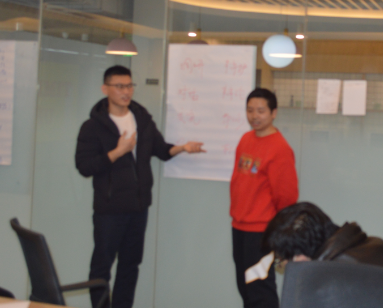
\includegraphics[width=6cm]{1499.png}\textbar{}辩解

\hypertarget{ux5982ux4f55ux5728ux8fedux4ee3ux56deux987eux65f6ux5206ux6790ux7f3aux9677ux6570ux636eux5f97ux51faux9884ux6d4bux6a21ux578bux53c2ux6570}{%
\subsection{如何分析缺陷数据得出预测模型参数,出分布图}\label{ux5982ux4f55ux5728ux8fedux4ee3ux56deux987eux65f6ux5206ux6790ux7f3aux9677ux6570ux636eux5f97ux51faux9884ux6d4bux6a21ux578bux53c2ux6570}}

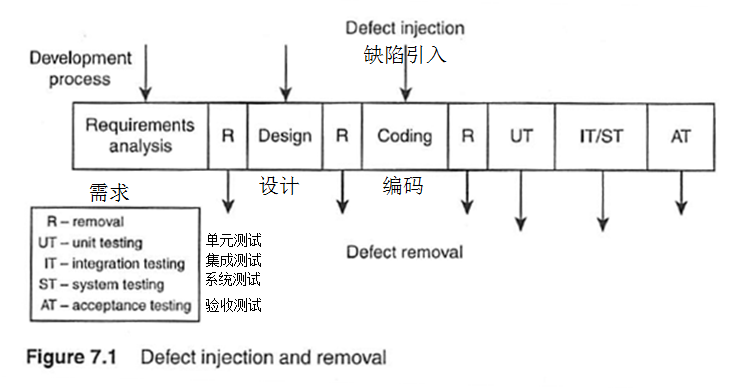
\includegraphics[width=6cm]{Jaloteemm110.png}

需求、设计、编码后都会评审/测试来排除缺陷,但仅仅做评审/测试不一定能确保质量。因为最终验收缺陷数取决于每个步骤能否有效排除当前的缺陷。\\

可以用缺陷排除率(Defect Removal Efficiency DRE) 来衡量测试或评审的效率:


%\href{文件:Ma3_1.0.png}{文件:Ma3 1.0.png}

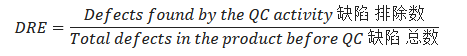
\includegraphics[width=6cm]{Ma3_10.png}

有些人会认为尽早发现并解决缺陷

对质量肯定好,但会耗费工作量,增加项目成本,老板不一定愿意。

其实是反过来,如能在前面预先发现并修正缺陷,

便能减小后面测试和修改缺陷的工作量,

最终只会减少总项目工作量。

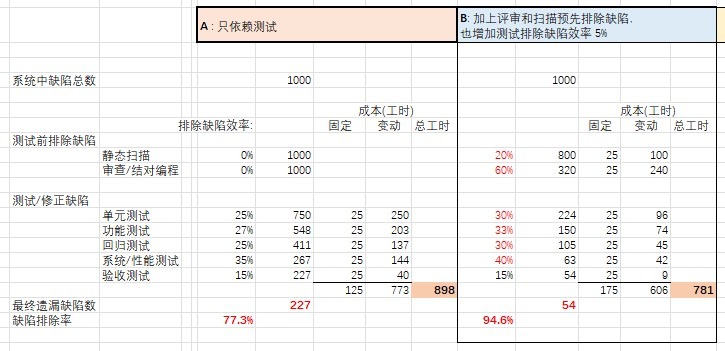
\includegraphics[width=6cm]{AR1FixVarCostScreenshot_2022-12-10_144400.jpg}

比较以上两种策略的质量成本(COQ)就能看出:

\begin{itemize}
\tightlist
\item
  增加测试前扫描与审查,并加大测试效率,不仅减少最终缺陷数到54(对比227),也降低总质量成本(总人时)
\end{itemize}

\framebox{%
\begin{minipage}[t]{0.97\columnwidth}\raggedright
假设:每项任务的固定成本都是25人时;测试前的缺陷修复:每缺陷用
0.5人时;测试缺陷修复,上面计算假定每缺陷用1人时,详见下表:

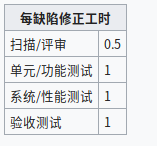
\includegraphics[width=6cm]{Screenshotfrom2023-11-0302-29-26.png}
%Screenshotfrom2023-11-0302-29-26.png

%通常测试里的缺陷修复每缺陷不只一人时,例如,在验收阶段时可能要用20人时;我通常会打开这XLS
%表,填上客户的估计值。从上表看到,即使用最少的1人时来算,还是不亏。

\begin{itemize}
\tightlist
\item
  通常测试里的缺陷修复每缺陷不只一人时,例如,在验收阶段时可能要用20人时;我通常会打开这XLS
表,填上客户的估计值。从上表看到,即使用最少的1人时来算,还是不亏。
\end{itemize}

\strut
\end{minipage}}

因为缺陷已经提前被排除系统测试的缺陷减少,测试阶段的工作量减少大于前面扫描评审上的投入。

可以进一步利用COQ概念,增加早期预防缺陷措施,如用原型与客户交流,做好需求调研,进一步减少缺陷,和成本。
例如,使用原型与场景与客户挖掘需求,可进一步把缺陷降到43,也降低总质量成本:

%\href{文件:est缺陷表3.jpg}{600px}

\includegraphics[width=10cm]{est缺陷表3.jpg}\\

\texttt{注:你可能会质疑使用原型方法不只25人时,但即使加大到100人时,还是不亏。因它能预防缺陷,整体缺陷数下降20\%,使总质量成本下降超过100人时。}


下面我们介绍一下怎么从引进量化管理来提高开发质量:\\
\#设定量化目标。例如希望最终遗漏到验收发现的缺陷数降多少?

\begin{enumerate}
\tightlist
\item
  并设定中间阶段目标缺陷数,从而预测能否达到最终目标,不要等到最后才知道不满足
\end{enumerate}

可用缺陷排除率来判断每一个过程的质量:\\
如果要最终质量好,缺陷排除率就要高。但计算缺陷排除率,必须要等到整个开发完成才可以计算,我们可以建立一个预测模型,模拟这个过程:\\
需求会引入缺陷,然后需求评审排除缺陷等等。把各引入缺陷数,排除率输进蒙地卡罗预测模型,然后使用它估计每个阶段的缺陷数量范围。

Table 7.2 Defect Distribution in Infosys's PCB Infosys PCB的缺陷分布

%Screenshotfrom2023-10-1023-46-22.png

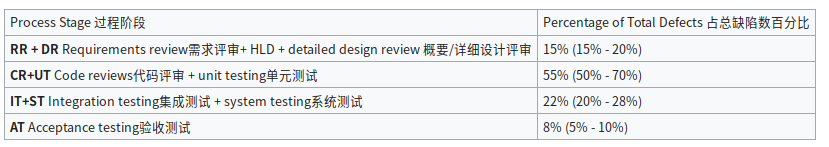
\includegraphics[width=6cm]{Screenshotfrom2023-10-1023-46-22.png}

如果我们按上面 infosys
公司的各阶段缺陷利率百分比,设计与需求排除缺陷15\%,代码评审与单元测试55\%,集成/系统测试22\%,验收测试8\%,下面按缺陷总数为100,
得出算出设计与需求排除共15缺陷, DR+RR=15,CR+UT=55, IT+ST=22,
AT=8,求出各阶段的缺陷输入与缺陷排除率,把参数输入蒙地卡罗预测模型:\\
表D1:\\
%\href{文件:1113correctEgScreenshot_2021-11-13_212414.png}{400px}
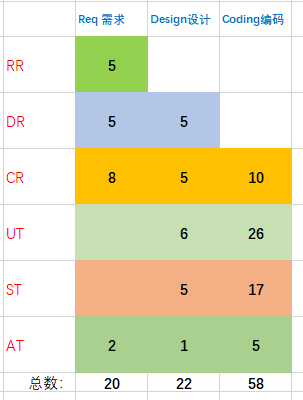
\includegraphics[width=6cm]{1113correctEgScreenshot_2021-11-13_212414.png}

%\href{文件:1113corrDreScreenshot_2021-11-13_212509.png}{600px}
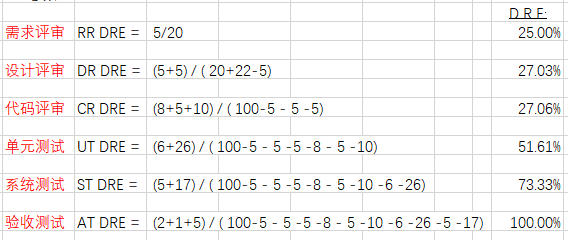
\includegraphics[width=6cm]{1113corrDreScreenshot_2021-11-13_212509.png}

得出下面Figure7.2,缺陷分布是中间最高头尾低,右面与左面不同,有条长尾巴,类似估算软件开发项目工作量的
Rayleigh 曲线。

%\href{文件:jalote_emm_7.2.png}{500px}
\includegraphics[width=6cm]{jalote_emm_72.png}

模型假定每个阶段的缺陷排除率都比较稳定,在某个范围之内,不同阶段引入的缺陷也在一定范围之内。
蒙地卡罗模型让我们可以设定缺陷排除率和缺陷输入数量的波动范围,预测各阶段缺陷排除分布范围,不仅仅看单点数(前面在第三章里介绍过如何使用蒙地卡罗模型做三点估算)。

\hypertarget{ux57f9ux8badux5bf9ux8c61}{%
\subsubsection{使用水晶球蒙地卡罗模型实例}\label{ux57f9ux8badux5bf9ux8c61}}

\begin{itemize}
\tightlist
\item
  在模型参数输入部分输入估计对应缺陷排除百分比的上下限与均值,工作量也类似。例如,代码走查的缺陷排除率是55%;评审工作量(不包含修正缺陷)为20人时。如代码正式审查排除率是85%,但工作量会增加到35人时 。如下图:

\end{itemize}

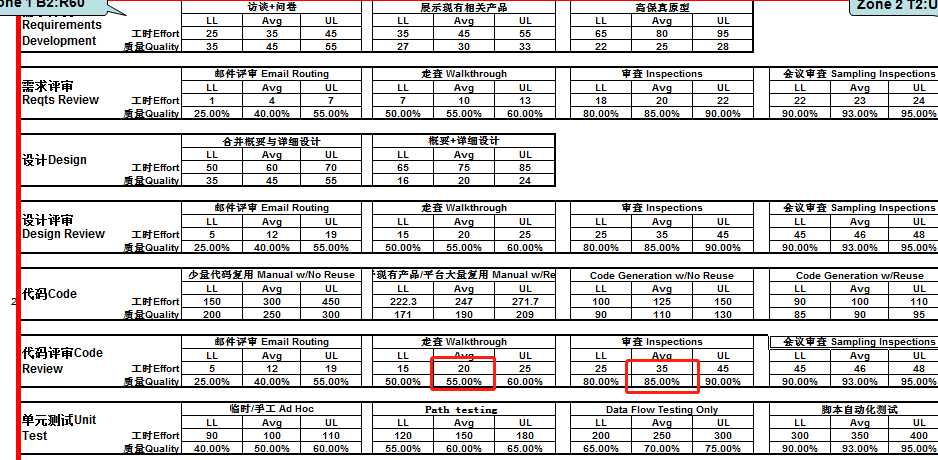
\includegraphics[width=6cm]{微信截图_20211027011246.png}

\begin{itemize}
\tightlist
\item
  模型会自动按输入的最大最小值用PERT方程式计算标准差,变成分布(正态(normal)分布、),水晶球模型会依据 Decision 格的数字选取对应的分布,

\end{itemize}

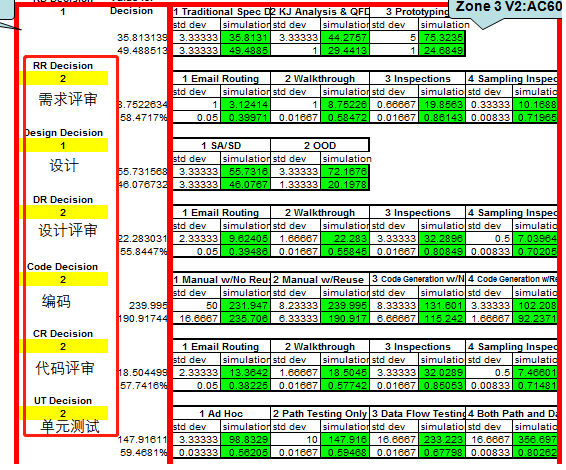
\includegraphics[width=6cm]{微信截图_20231027140307.png}

\begin{itemize}
\tightlist
\item
  成本参数:例如 Quality 行:修复一个系统测试发现的缺陷,平均要用8000元,最高9200,最低6800。例如 Effort 行:平均人时成本,平均是600元,最750,最低500。水晶球模型就会依据输入依据三角形分布估算单位成本的分布,放在绿格里。
\end{itemize}

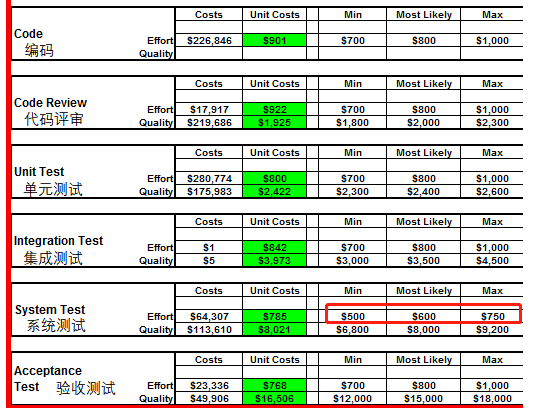
\includegraphics[width=6cm]{微信截图_20231027140341.png}

\begin{itemize}
\tightlist
\item
  估算质量成本:水晶球会依据质每过程的缺陷分布和单位成本分布,预估质量成本的分布。例如这例子是需求评审用审查(2),设计评审用走查(2) ,代码评审也用走查(2),单元测试是手工(1),系统测试估计走3轮(2),验收测试预计走3轮(2)的预估分布结果。(括号里的数字代表在模型参数表里那一栋,从1至4。如想了解水晶球如何把每个过程”加”起来,详见‘三点估算’附件:蒙特卡洛模拟)
\end{itemize}

\begin{itemize}
\tightlist
\item
  模型经过 10,000 次模拟得出质量成本分布,和过程的缺陷分布与范围(90\%置信区间)
\end{itemize}

\hypertarget{asch-1951-ux7fa4ux4f17ux538bux529bux5b9eux9a8c}{%
\subsection{Asch 1951
群众压力实验}\label{asch-1951-ux7fa4ux4f17ux538bux529bux5b9eux9a8c}}

%\href{文件:Asch0Screenshot_2022-07-09_161023.jpg}{150px}
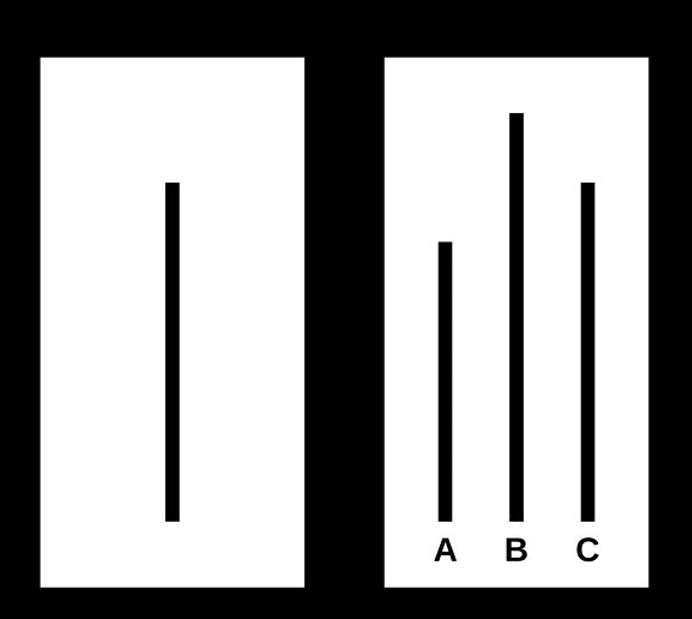
\includegraphics[width=6cm]{Asch0Screenshot_2022-07-09_161023.jpg}

问题:\textbf{请问右面那条线 (A, B, C) 的长度最接近左面线的长度?}

%\url{文件:Asch2Screenshot.2.png}
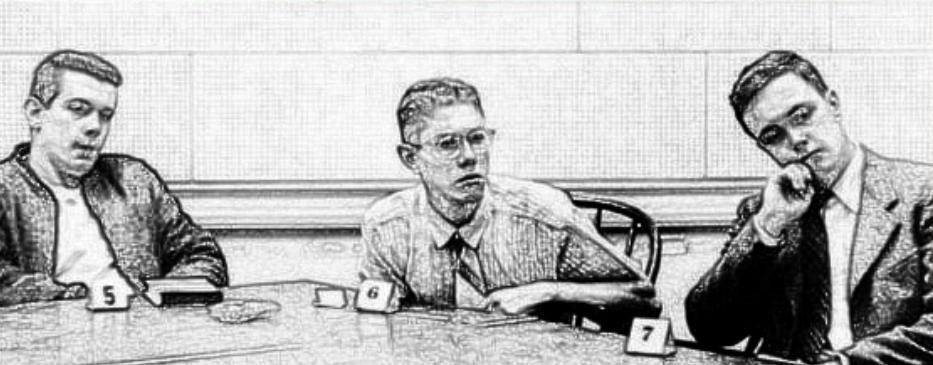
\includegraphics[width=6cm]{Asch2Screenshot2.png}

实验设计:\textbf{随机邀请几位志愿者(包括你)
参加,实验之前与(除了你以外)所有人预先说好,都选A,并且要假装成经过深思熟虑。实验时,你是最后一位作答。}

结果:

\begin{itemize}
\tightlist
\item
  有群众压力时,大概\textbf{37\%}会从众选择错误答案
  (虽然不同人有差异,但总体只有\textbf{25\%}能坚持自己的正确答案。)
\item
  个人自己作答,接近100\%选对,错误率\textbf{少于1\%}
\end{itemize}

影响因素:

\begin{itemize}
\tightlist
\item
  前面选择错误答案的人数越多,错误率越高:
\end{itemize}

\begin{enumerate}
\tightlist
\item
  一位:接近0\%答错
\item
  两位:大概14\%
\item
  三位: 32\%(详见下图)
\end{enumerate}

%\href{文件:Asch3Screenshot_2022-07-08_201341.1.png}{500px}
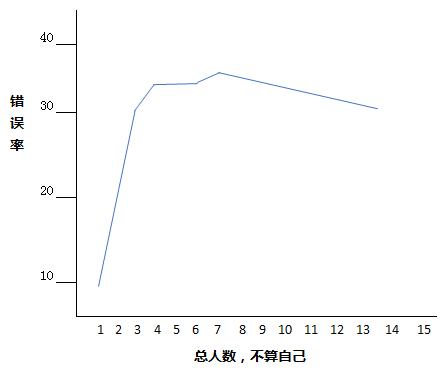
\includegraphics[width=6cm]{Asch3Screenshot_2022-07-08_2013411.png}

\begin{itemize}
\tightlist
\item
  如果前面有一位``战友''选了正确答案,你的错误率就显著降低(大约原本水平的1/4,看下图黄线),并让你感到与他更亲切
\end{itemize}

%\href{文件:Asch4Screenshot_2022-07-08_201502.1.png}{500px}
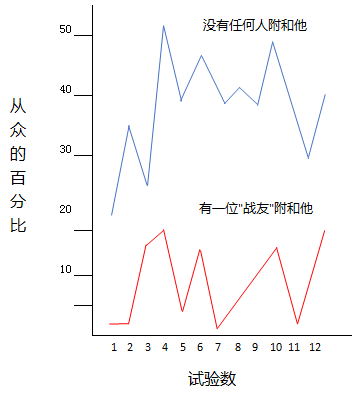
\includegraphics[width=6cm]{Asch4Screenshot_2022-07-08_2015021.png}

\begin{itemize}
\tightlist
\item
  尴尬场景(例如迟到),你的错误率会更高。

  \begin{itemize}
  \tightlist
  \item
    实际你没有晚到,只是让你觉得确实迟到了,觉得尴尬。
  \end{itemize}
\item
  如果不是要你说出答案,而是让你把答案写在纸上,错误率会降低三分之一。
\end{itemize}

\hypertarget{brehm-1956-ux51b3ux7b56ux5f71ux54cdux5b9eux9a8c}{%
\subsection{Brehm 1956
决策影响实验}\label{brehm-1956-ux51b3ux7b56ux5f71ux54cdux5b9eux9a8c}}

\textbf{实验设计}:

\begin{enumerate}
\tightlist
\item
  提供十多种不同礼物,包括台灯,多士炉,挂钟、收音机等。
\item
  请你按自己喜好对礼物排序
  。例如最喜欢的选一,如果同样喜欢两件礼物,可以不分高低,写同一个数字。
\item
  让你从两件同样喜好的礼物,让你选其中一件,让你拿走。
\item
  但在你离开之前,请你再对所有礼物按喜好排序。
\end{enumerate}

\textbf{结果}:

\begin{itemize}
\tightlist
\item
  绝大部分人都会抬高自己选择拿走的那一件礼物排序,调低非选择的那件礼物排序。
\item
  但如果不是自己选择,而是由老师选好给你,你后面的礼物排序就没有变化。
\end{itemize}

\textbf{结论}:

\begin{itemize}
\tightlist
\item
  人都会觉得自己的选择比较好。
\item
  例如选大学、选汽车、选伴侣。如果是由你自己决定选择(非被安排),你会不会都会觉得自己的选择较好。
\end{itemize}

\hypertarget{ux7caeux98dfux5206ux914dux5b9eux9a8c}{%
\subsection{粮食分配实验}\label{ux7caeux98dfux5206ux914dux5b9eux9a8c}}

二战时,美国虽然不是战区,也需要控制粮食供应。政府面对的难题:

\begin{itemize}
\tightlist
\item
  怎么让那些家庭的消费习惯,满足战时的食物供应。
\end{itemize}

比如当时有些食物是要分配的,如何让家庭多吃一些供应充足的食物,避开紧缺的食物。他们实验发现,首先要知道整个过程是家庭里哪个人做这一块的决定。\\
研究分析发现,绝大部分的家庭都是由家庭主妇决定购买什么、储存什么、怎么做菜,丈夫没有太多的意见,通常是由媳妇决定。

\textbf{实验设计}:

\begin{itemize}
\tightlist
\item
  把家庭主妇分成两组:
\end{itemize}

\begin{enumerate}
\tightlist
\item
  专家跟一组家庭主妇宣扬某种食物营养丰富,对家人的身体都会有好处。
\item
  另一组家庭主妇没有专家指导,只是给她一些营养的数据,邀请主妇分成小组自己讨论决定怎么去做.\\
\end{enumerate}

\textbf{结果}:实验发现第一种方法没有效果,第二种效果却很好。

\hypertarget{kjux5206ux6790ux65b9ux6cd5ux6b65ux9aa4}{%
\subsection{KJ分析方法步骤}\label{kjux5206ux6790ux65b9ux6cd5ux6b65ux9aa4}}

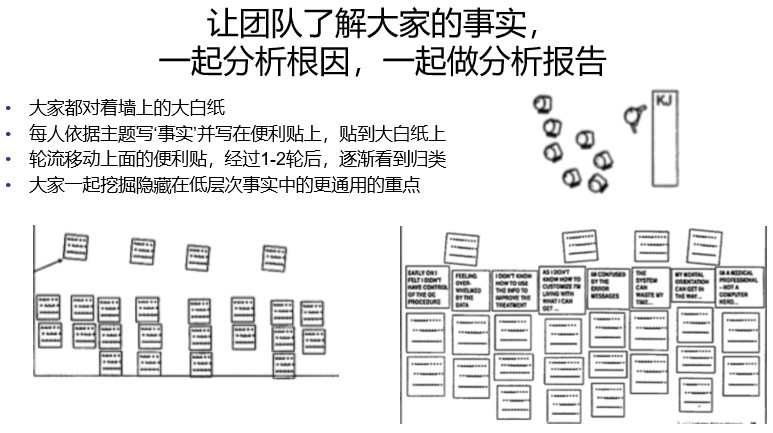
\includegraphics[width=6cm]{Kj1Screenshot2023-11-01133052.jpg}

\emph{一种头脑风暴方法,每人把自己想法写在便利贴上,一起轮流把所有便利贴排放分组}

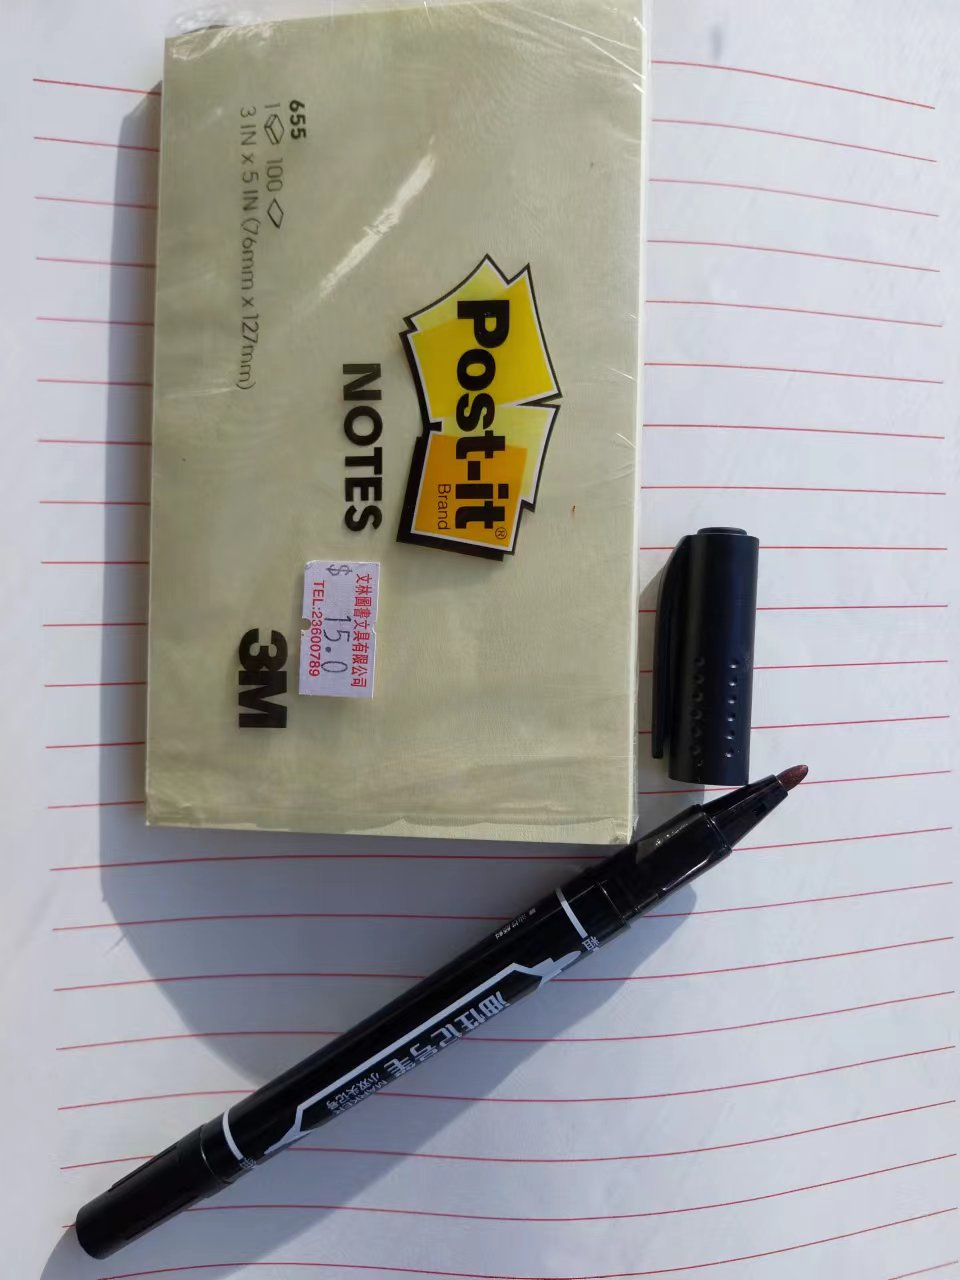
\includegraphics[width=6cm]{微信图片_20231027091622.jpg}

\includegraphics[width=6cm]{微信图片_20231027091728.jpg}

\begin{description}
\item[]
\begin{description}
\tightlist
\item[]
\end{description}
\end{description}

\begin{enumerate}
\tightlist
\item
  把主题以问题形式写在大白纸的头顶
\item
  把相关的事实写在便利贴上面,用黑色
\item
  搜集相关的事实,如果是一组人的话,分散到不同人手上
\item
  (团队)查看描述是否不清楚,是否要整理?
\item
  每人轮流把相关的便利贴组合在一起
\item
  当每人都已经调整过便利贴组合后,一起把每一组便利贴加上一个题目,用红色标识
\item
  红色的标题下包含相关事实的内容
\item
  把相关的红色题目(最好不超过3个)组合在一起
\item
  给这大组一个题目 -- 蓝色
\item
  在题目下放上相关的红色小组
\item
  把蓝色的题目和剩下红色的小组或单独没有分类的便利贴都在墙上放好,也可以用一些箭头描述它们的因果关系

\end{enumerate}


%\href{文件:KJ_1.0.png}{600px}
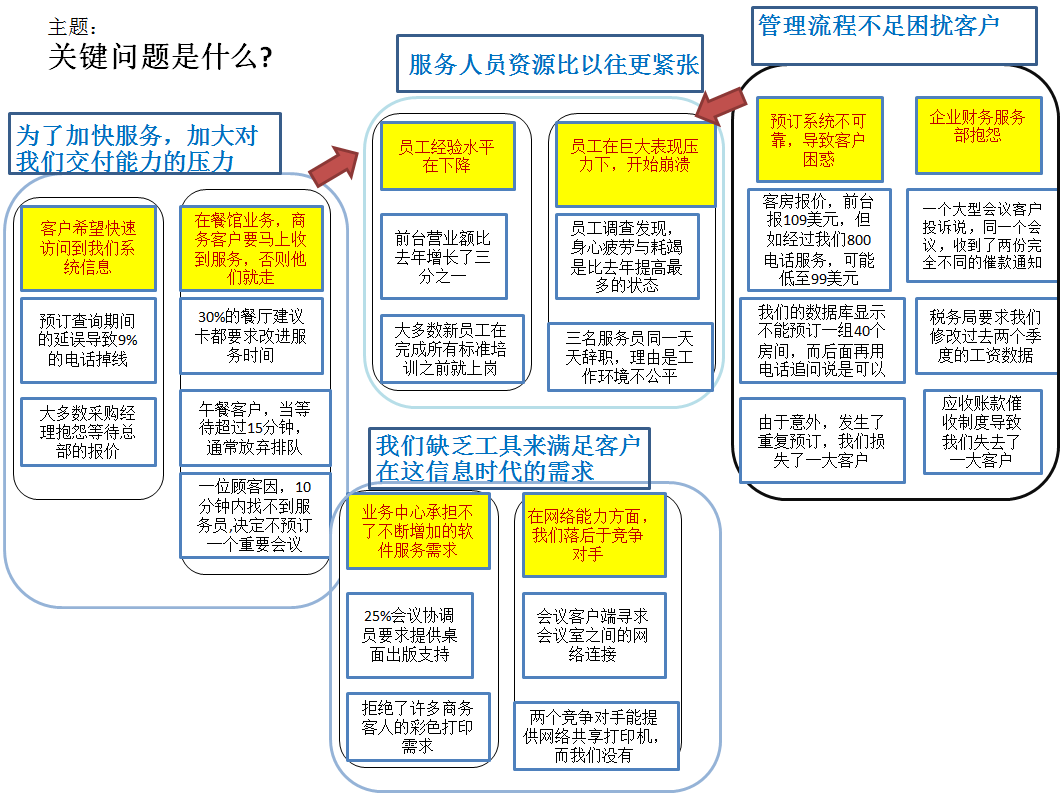
\includegraphics[width=6cm]{KJ_10.png}

\hypertarget{ux6c34ux6676ux7403ux8499ux7279ux5361ux6d1bux9884ux6d4bux6a21ux578b}{%
\subsection{水晶球蒙特卡洛预测模型}\label{ux6c34ux6676ux7403ux8499ux7279ux5361ux6d1bux9884ux6d4bux6a21ux578b}}

\begin{itemize}
\tightlist
\item
  在模型参数输入部分输入估计对应缺陷排除百分比的上下限与均值,工作量也类似。例如,代码走查的缺陷排除率是55%;评审工作量(不包含修正缺陷)为20人时。如代码正式审查排除率是85%,但工作量会增加到35人时 。如下图:
\end{itemize}

%\href{文件:微信截图_20211027011246.png}{450px}

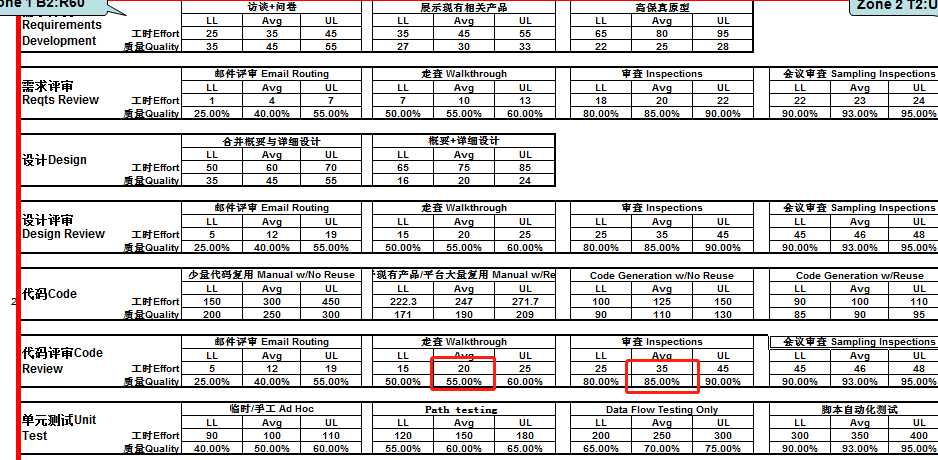
\includegraphics[width=6cm]{微信截图_20211027011246.png}

\begin{itemize}
\tightlist
\item
  模型会自动按输入的最大最小值计算标准差,变成分布(如:正态(normal)分布、三角形(triangular)分布),水晶球模型会依据黄格里的数字选取对应的分布,
\end{itemize}

%\href{文件:微信截图_20211027011403.png}{450px}

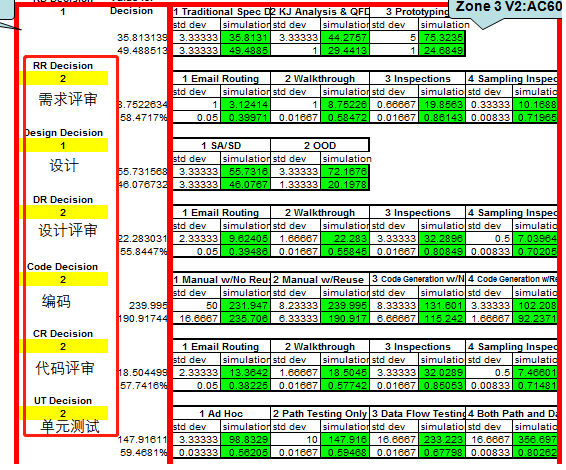
\includegraphics[width=6cm]{微信截图_20231027140307.png}

\begin{itemize}
\tightlist
\item
  成本参数:例如 Quality 行:修复一个系统测试发现的缺陷,平均要用8000元,最高9200,最低6800。例如 Effort 行:平均人时成本,平均是600元,最750,最低500。水晶球模型就会依据输入依据三角形分布估算单位成本的分布,放在绿格里。
\end{itemize}

%\href{文件:微信截图_20211027012006.png}{450px}

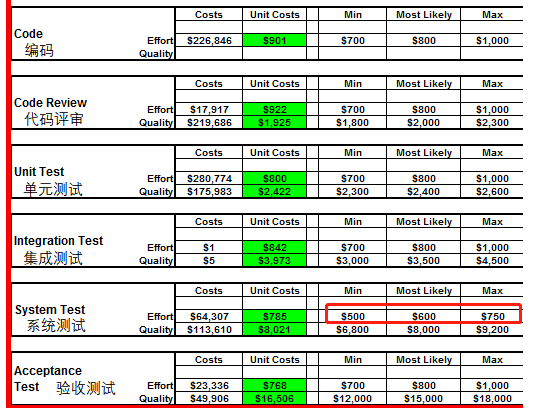
\includegraphics[width=6cm]{微信截图_20231027140341.png}

\begin{itemize}
\tightlist
\item
  估算质量成本:水晶球会依据质每过程的缺陷分布和单位成本分布,预估质量成本的分布。例如这例子是需求评审用审查(2),设计评审用走查(2) ,代码评审也用走查(2),单元测试是手工(1),系统测试估计走3轮(2),验收测试预计走3轮(2)的预估分布结果。(括号里的数字代表在模型参数表里那一栋,从1至4。如想了解水晶球如何把每个过程”加”起来,详见‘三点估算’附件:蒙特卡洛模拟)
\end{itemize}

\begin{itemize}
\tightlist
\item
  模型经过 10,000 次模拟得出质量成本分布,和过程的缺陷分布与范围(90\%置信区间)
\end{itemize}

%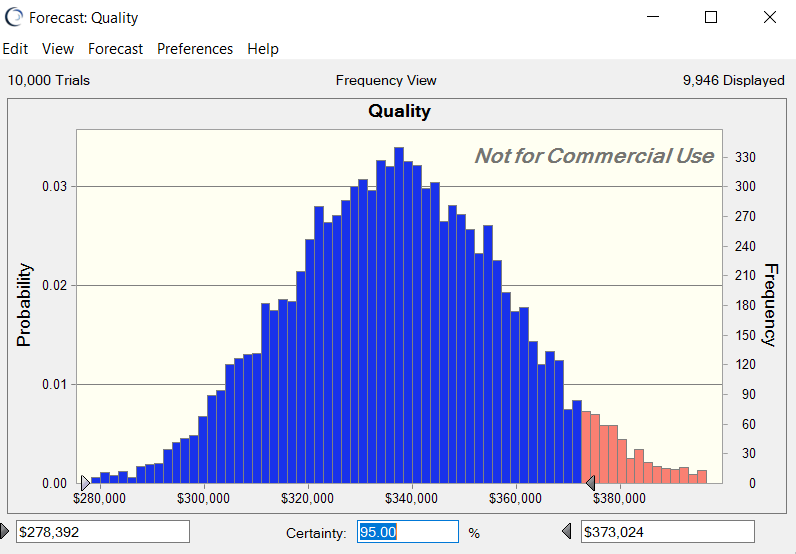
\includegraphics[width=6cm]{StartQUA95.PNG}
